\documentclass[12pt]{article}
\usepackage[margin=1in]{geometry}

\usepackage{setspace}
\doublespacing

\usepackage{graphicx}

\title{The acquisition metaphor (for morning people)}
\author{Colby Goettel}

\begin{document}
\maketitle

% Prompt: Describe in your own words the two metaphors for learning presented in Sfard's article "On Two Metaphors for Learning and The Dangers of Choosing Just One." Be sure to clarify how the two metaphors differ and why that difference is significant. (That is, what's the debate about?) Finally, from your perspective, what is the advantage or disadvantage of having both metaphors (and possibly others) in the discipline of education? Defend your answer.

% DEFINE AM
% Learning
% Concepts build on each other (justified?)
% Fact-based
% Memory. Information is stored (yeah, duh).
The acquisition metaphor (AM) is a convoluted way of saying that people learn by learning (as opposed to doing). Facts, ideas, and concepts build on each other. These pieces of information~--- objects~--- are what is known as knowledge. Knowledge is then internalized and stored in memory. Historically, AM has been the metaphor used for thousands of years to describe knowledge and learning. Generally, when people think about learning, they think AM.

% DEFINE PM
% Doing
% It's not something we have, it's something we do
% social, cultural
% hippie dippie being a part of something
% part of a community (hardcore/punk/ska/skinhead?)
% all-encompassing
The participation metaphor (PM) is a learning style dictated by actions: people learn by doing. PM advocates teach that knowledge is not something that people have, it's societal and communal. Learning is done by being part of a community. This type of learning is all-encompassing~--- learning isn't something that anyone has, it's one part of the whole.

% CONTRAST AM AND PM. What's the debate about?
% AM: mind. facts. knowledge (as generally understood).
% PM: bonds between people and things
% AM: internalization of knowledge
% PM: all-encompassingness of ideas
Proponents of AM and PM have formed into camps, warring with each other about which is the True and Living Metaphor to describe learning. I firmly believe that this so-called debate is artificial, created for the sake of argument. It allows each side to better understand themselves. AM and PM focus on two completely different aspects of learning. They're definitely related, but they also exist independently. These metaphors are symbiotic and thrive on each other.

Knowledge, neurologically speaking, is when the myelin sheaths of neurons form along certain pathways, making memory. These memories, like muscle, are reinforced as they are used and weaken when not.

In another sense, knowledge is only gained by being part of a community. Whether that be the chess club, a math class, or on a national or global level, these are all communities in which individuals learn and form memories.

% DISADVANTAGES OF HAVING BOTH
PM argues that no knowledge is centrally held, but is communal. True, but it's 2015: there is no longer this primal sense of community in the world. Technology has bridged that gap and allowed individuals to join whichever communities they'd like. Go to a library and join the other communities by reading their literature. E-mail a professor and ask questions. It's odd that people are arguing PM in light of all the technological advances that seem to make it obsolete (or, at least, in need of some serious revision).

% ADVANTAGES OF HAVING BOTH
% PM is the stupidest argument I've ever read. No freaking duh you learn in a societal way, BUT THEN YOU INTERNALIZE THOSE CONCEPTS.
% "objectifying knowledge"? Are you kidding me?
In reality, it seems that these metaphors are actually a methodology: first, an individual learns in a community (PM), but then internalizes that knowledge (AM). PM has it wrong that knowledge is some hippie-dippie, nebulous thing that exists but doesn't really exist and was created \textit{ex nihilo}: it's facts and concepts and ideas and strategies and methodologies that are taught to people in a society and are then propagated through language and actions. These knowledge objects are then internalized and stored in the individual's memory (AM) and in the memory of the community (PM).

% CONCLUSION
These metaphors exist in harmony. People have created an artificial debate because it helps them learn. Both metaphors exist. Everyone has experienced both in their lives because that's how the world works.

\clearpage
\begin{center}
    {\LARGE Information processing}
\end{center}
% Prompt: Describe the classic information-processing (i.e., Atkinson and Shiffrin) model. What are its components and how does it work? (You can add updated understandings as well, regarding working memory, forgetting, etc.) In what sense is this a model of human learning? In other words, what does learning involve from this perspective?

% DEFINE
The Atkinson-Shiffrin model of memory is shown in Figure~\ref{fig:memory-model}. The premise is that as individuals pay attention to sensory stimulation, short-term memories are created. As short-term memory is rehearsed and transferred, it turns into long-term memory. As long-term memory is retrieved, it comes into short-term memory so that it can be used.

\begin{figure}[h]
    \centering
    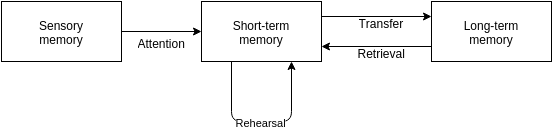
\includegraphics[width=0.65\textwidth]{memory-model}
    \caption{The Atkinson-Shiffrin model of memory.}
    \label{fig:memory-model}
\end{figure}

% COMPONENTS/HOW IT WORKS
The major components of this model are some form of input, storage, retrieval, and (eventually) forgetting. When presented with information, an individual must input and store the information. This creates short-term memory. If this memory is rehearsed (retrieved) often, it has a chance to become long-term memory. Neurologically speaking, when memories are rehearsed, the myelin sheaths of neurons form along certain pathways making memory. However, like muscle, if these memories are not used, they are lost.

% WHAT ARE SHORT-TERM AND LONG-TERM MEMORY?
There are limits to short-term memory, though. Miller defined short-term memory as being limited to $7\pm2$ items. The base number, 7, can be increased slightly through training, but it is always limited. In contrast, there is no limit on long-term memory.

% HOW IS THIS A MODEL OF HUMAN LEARNING?
This model works as a basic model of human learning because learning is the internalization of knowledge in long-term memory. It must be able to be retrieved. If an individual has successfully internalized and retrieved knowledge, they have learned. In education, this is the predominant reason why exams exist. Exams test students to see if they have learned the concepts taught in a class. The first midterm in your 629 class is actually a really great example of the difference between memorization and internalization. The two questions presented as possible exam questions approached the material in fundamentally different ways. The second question asked for a presentation of the facts from the class. It was obvious that this would not be the question selected for the midterm because it was only asking for a rote rehearsal and recitation of ideas. The first question, however, was a deeper question because it wasn't looking merely for facts, but to see if the students had internalized the concepts, making them their own. It was an application-based question.

% HOW DOES THIS RELATE TO LEARNING?
With this in mind, we ask ``What is learning?'' Is learning the mere memorization of methodologies, or is it the internalization of ideas? Look at the readings students do for a course: what does it mean to do 100\% of the reading for a course? Does it mean that a student has read every word assigned? What if they skim the reading, but learn 100\% of the material? If this reasoning is taken to the other extreme, what if a student doesn't do any reading, but understands 100\% of the material? Surely there is a correlation between reading and understanding, but that doesn't mean that students have to read every single word in order to understand the concepts. In fact, what about the student who reads every word but doesn't internalize and understand the concepts? They've read every word, but they haven't accomplished the purpose behind the readings. So have they really done the readings?

% FROM THIS PERSPECTIVE, WHAT DOES LEARNING INVOLVE?
From this perspective, it's easy to see that learning cannot simply be the memorization of facts. Memorization is necessary, but not sufficient. A student must internalize concepts and be able to apply them in various fields. The concept of transfer comes into play here: if a student cannot transfer knowledge, they have not properly learned it yet. They might have a rudimentary understanding of the material, but they haven't truly learned.

% CONCLUSION
The Atkinson-Shiffrin model of memory shows the basic process by which people store information, but lacks the depth necessary to properly portray pedagogy. Learning is more than memorization: it's internalization and application.

\end{document}
